\documentclass[11pt]{article}
\newcommand{\blind}{1}

\usepackage[nodisplayskipstretch]{setspace}
\setstretch{1}

\usepackage[utf8]{inputenc}
\usepackage{lipsum}

\usepackage{amsmath,amssymb}
\usepackage{natbib}


\usepackage{amssymb,amsbsy,amsfonts,amsmath,xspace,amsthm}
\usepackage{mathrsfs}
\usepackage{graphicx}
\allowdisplaybreaks

\usepackage{caption}
\usepackage{setspace}
\usepackage{comment}
%\doublespacing
\usepackage[margin=1in]{geometry}
\usepackage{enumitem} 
\usepackage{subcaption}
\usepackage{multirow}
\usepackage{epstopdf}
\usepackage{epsfig}
\usepackage[colorlinks,citecolor=blue]{hyperref}

\usepackage[labelfont=bf]{caption}
\usepackage{url}
\usepackage[toc,page]{appendix}
\usepackage{float}
\usepackage{natbib}
\usepackage{color}
\usepackage[dvipsnames]{xcolor}
\usepackage{verbatim}
\usepackage{authblk}
\usepackage[normalem]{ulem}


\def\ack{\section*{Acknowledgements}%
  \addtocontents{toc}{\protect\vspace{6pt}}%
  \addcontentsline{toc}{section}{Acknowledgements}%
}


\usepackage{hyperref}
\hypersetup{
    colorlinks=true,
    linkcolor=blue,
    filecolor=magenta,      
    urlcolor=cyan,
    citecolor=blue
}
 
 


\usepackage{amsmath}
\usepackage{graphicx}
\newcommand*{\KeepStyleUnderBrace}[1]{%f
\mathop{%
\mathchoice
{\underbrace{\displaystyle#1}}%
{\underbrace{\textstyle#1}}%
{\underbrace{\scriptstyle#1}}%
{\underbrace{\scriptscriptstyle#1}}%
}\limits
}
\usepackage{mathtools}
\mathtoolsset{showonlyrefs}
\usepackage{amsmath,amssymb,amsthm,bm,hyperref}
\usepackage{dsfont,listings}

 \renewcommand\footnotemark{}

\usepackage[ruled,vlined]{algorithm2e}
\SetAlFnt{\small}
\SetAlCapFnt{\small}
\SetAlCapNameFnt{\small}

\newtheorem*{theorem*}{Theorem}
\usepackage{enumitem}
\theoremstyle{plain} 
\newtheorem{thm}{Theorem}
\newtheorem{lem}{Lemma}

\theoremstyle{definition}
\newtheorem{prop}{Proposition}
\newtheorem{corollary}{Corollary}
\newtheorem{assumption}{Assumption}
\newtheorem{defn}{Definition}
\newtheorem{example}{Example}
\newtheorem{rmk}{Remark}


\usepackage{xcolor}
\allowdisplaybreaks
\input macros.tex

\setcounter{secnumdepth}{3}

\def\spacingset#1{\renewcommand{\baselinestretch}%
{#1}\small\normalsize} \spacingset{1}
\def\fixme#1#2{\textbf{\color{red}[FIXME (#1): #2]}}
\def\mycomment#1{\textbf{\color{blue}#1}}
\def\ccomment#1{\textbf{\color{ForestGreen}#1}}
\usepackage{hyperref}
\usepackage[parfill]{parskip}
\usepackage{bm}


\newcommand{\Hnorm}[1]{\left\lVert#1\right\rVert_{\tH_\alpha}}
\newcommand{\nullnorm}[1]{\left\lVert#1\right\rVert}
\def\trueB{\mB^{\text{true}}}
\def\newX{\mX_{\textup{new}}}
\def\newy{y_{\textup{new}}}
\def\sign{\textup{sign}}
\def\bayesf{f_{\textup{bayes}}}
\def\bayesS{S_{\textup{bayes}}}
\def\bayespif{f_{\textup{bayes},\pi}}
\def\CNN{\text{\bf \small CNN }}
\def\Lasso{\text{\bf \small Lasso }}
\def\NonparaM{\text{\bf \small NonMAR }}
\def\LogisticM{\text{\bf \small LogisticM }}
 
 

\usepackage{setspace}
\onehalfspacing
 
\begin{document}


\section*{Appendix}
\addcontentsline{toc}{section}{Appendices}
\renewcommand{\thesubsection}{\Alph{subsection}}
\setcounter{figure}{0}
\setcounter{table}{0}
\renewcommand{\thetable}{S\arabic{table}}
\renewcommand{\thefigure}{S\arabic{figure}}
\renewcommand{\figurename}{Supplemental Figure}
\renewcommand{\tablename}{Supplemental Table}


\subsection{Connection to joint matrix decomposition with functional coefficients}\label{sec:joint}
In the main text, we have shown that our classifier functions $\tF(r,s_1,s_2)$ incorporates certain retrospective models $\mX|y$. Here we extend the retrospective model to a more general family  which we coin as ``functionally decomposable matrices''. The model essentially extends Example~\ref{example2} from two classes of $\mX$ to a series of $\mX$ on a continuous spectrum of $\pi$. 

\begin{example}[Functionally decomposable matrices]\label{ex:matrix_decomposition}
We consider a matrix model $\mX_\pi\stackrel{\text{def}}{=}\mB_0+ \sum_{s\in[r]}g_s(\pi)\mB_s+\sigma \mE$, where $\pi \in[0,1]$ is a real-valued index; $\mE$ is a noise matrix consisting of i.i.d.\ entries in $N(0,1)$; $\sigma$ is the noise level; $\mB_0$ is an arbitrary baseline matrix; $(\mB_s)_{s\in[r]}$ is a set of rank-1 matrices in $\{0,1\}^{d_1\times d_2}$ that satisfy (i) non-overlapping supports, i.e., $\langle \mB_s, \mB_{s'}\rangle=0$ for all $s\neq s'$, and (ii) bounded total support, i.e., $\sum_{s\in[r]}\text{supp}(\mB_s)\leq (s_1,s_2)$; and the coefficients $g_s(\cdot)\colon [0,1]\to\mathbb{R}$ are monotonic functions with respect to $\pi$ for all $s\in[r]$. 

Now, suppose the observation takes the form of pair $(\mX_\pi,y_\pi)$ with $y_\pi \sim \text{Ber}(\pi)$, where $y_\pi$ is conditionally independent of $\mX_\pi$ given $\pi$, and $\pi\in[0,1]$ is drawn from an unknown distribution over $[0,1]$. Equivalently, the generative model is expressed in the following scheme:
\[
\pi \stackrel{\text{i.i.d.}}{\sim} \text{Uniform}[0,1] \stackrel{\text{conditional on $\pi$}}{\longrightarrow}
\begin{cases}
y\sim \text{Ber}(\pi),\ y\perp \mX|\pi, \\
\mX=\mB_0+\entry{\mX_{pq}},
\end{cases}
\]
where $ \mX_{pq}\stackrel{\text{indep.}}{\sim}\tN(g_{s}(\pi), \sigma^2)$ if  the position $(p,q)$ falls in the support of $\mB_s$ and $ \mX_{pq}\stackrel{\text{indep.}}{\sim}\tN(0,\sigma^2)$  otherwise.  Recall that $\mu(\mX)=\mathbb{E}(y|\mX)$. In the noiseless case $\sigma = 0$, there exists a sequence of functions $(f_\pi)_{\pi\in(0,1)}$ with $f_\pi \in\tF(r,s_1,s_2)$, such that $\sign (\mu(\mX)-\pi) = \sign f_\pi(\mX)$ for all $\pi \in (0,1)$.

The above example shows the connection of our method to joint decomposition of matrices $(\mX_\pi)_{\pi\in[0,1]}$. We should point out, despite of the seeming similarity, a fundamental challenge arises in our setting when the latent index $\pi$ is unobserved. Our level-set approach essentially learns the right ``sorting'' of $\mX_\pi$ against the index $\pi\in[0,1]$ (see Figure~\ref{fig:method}), thereby facilitating the joint estimation of matrix basis $\mB_s$ and relationship $\pi=\pi(\mX)$. 
\end{example}


Furthermore, we provide additional results on the low-rank two-way sparse classifiers. The following proposition gives a sufficient condition for exact recovery of level sets through halfspaces.
%; the results show that what essentially matters is the boundary of level sets.  where $S(\pi)$ be the level set defined in~\eqref{eq:level} and $\bar S(\pi)$ be the classifier defined in~\eqref{eq:optimization} optimized over $\tF(r,s_1,s_2)$. 

\begin{prop}[Low-rank and sparse boundaries]\label{prop:px} Let $\mu(\mX)$ be a regression function continuous in $\mX\in\mathbb{R}^{d_1\times d_2}$. Suppose that there exists a low-rank two-way sparse matrix $\mB_\pi$ and a real value $b_\pi\in\mathbb{R}$, such that the boundary set $\partial S(\pi)=\{\mX\colon \mu(\mX)=\pi\}$ is included in the set $\{\mX\colon \langle \mX, \mB_\pi \rangle = b_\pi\}$. Then $\sign (\mu(\mX)-\pi)=\sign (f_\pi(\mX))$ for some $f_\pi(\mX)\in \tF(r,s_1,s_2)$. Note that $(\mB_\pi, b_\pi)$ is allowed to vary depending on $\pi$. 
\end{prop}

\begin{proof}[Proof of Proposition~\ref{prop:px}]
For given $\pi\in\Pi$, suppose $\partial S(\pi) = \{\mX\colon \mu(\mX) = \pi\} = \{\mX:\langle \mB_\pi,\mX\rangle = b_\pi\}.$
Define two open sets $S_1$ and $S_2$ as 
\begin{align}
S_1(\pi) = \bar S(\pi)\setminus \partial S(\pi) = \{\mX\colon \langle \mB_\pi,\mX\rangle >b_\pi\}\quad\text{ and }\quad S_2(\pi) = \bar S^c(\pi) = \{\mX\colon \langle \mB_\pi,\mX\rangle < b_\pi\}.
\end{align}

First, we prove that there is no $\mX_1,\mX_2\in S_i(\pi)$ such that $p(\mX_1)>\pi$ while $p(\mX_2)<\pi$ for $i = 1, 2.$ To be specific, $S_i(\pi)$ is included either $S(\pi)\setminus\partial S(\pi) = \{\mX\colon \mu(\mX)>\pi\}$ or $S^c(\pi) = \{\mX\colon \mu(\mX)<\pi\}.$ 

It suffices to show the case $S_1(\pi)$.
Without loss of generality, suppose that there is $\mX_1,\mX_2\in S_1(\pi) $ such that $p(\mX_1)>\pi$ and $p(\mX_2)<\pi$. 
We can always find $\mX_3 = \lambda \mX_1+(1-\lambda)\mX_2$ for some $\lambda\in(0,1)$ such that $p(\mX_3) = \pi$ by continuity of $\mu(\mX).$ Because $p(\mX_3) = \pi$, we have  $\mX_3\in \partial S(\pi) = \{\mX\colon \mu(\mX) = \pi\} =  \{\mX\colon\langle \mB_\pi,\mX\rangle = b_\pi\}$. However, this contradict the fact \[\langle \mB_\pi,\mX_3\rangle =\lambda \langle \mB_\pi,\mX_1\rangle + (1-\lambda)\langle \mB_\pi,\mX_2\rangle> \lambda b_\pi+(1-\lambda)b_\pi = b_\pi. \]
Therefore, there is no $\mX_2\in\bar S_1(\pi)$ such that $p(\mX_1)<\pi$. 

Second, we prove that there are only two cases that 
\begin{enumerate}
    \item[(C1):]$S_1(\pi) = \{\mX\colon \mu(\mX) >\pi\} \text{ and } S_2(\pi) = \{\mX\colon \mu(\mX) <\pi\}$.
    \item[(C2):]$S_1(\pi) = \{\mX\colon \mu(\mX) <\pi\} \text{ and } S_2(\pi) = \{\mX\colon \mu(\mX) >\pi\}$.
\end{enumerate}
Suppose $S_1(\pi)\subset \{\mX\colon \mu(\mX)>\pi\}$. Since $\{\partial S(\pi),S_1(\pi),S_2(\pi)\}$ is a partition of $\mathbb{R}^{d_1\times d_2}$ and both $\{\mX\colon \mu(\mX)>\pi\}$ and $\{\mX\colon \mu(\mX)<\pi\}$ are non-empty set, only possible case is (C1). Similarly, if $S_2(\pi) \subset\{\mX\colon \mu(\mX)<\pi\}$, only possible case is (C2).

Notice that (C1) is equivalent to $S(\pi) = \bar S(\pi)$ while (C2) is equivalent to $S(\pi) = \bar S^c(\pi).$
\end{proof}



\clearpage
\subsection{Supplementary figures}\label{sec:sfigure}
     \begin{figure}[ht]
    \centering
    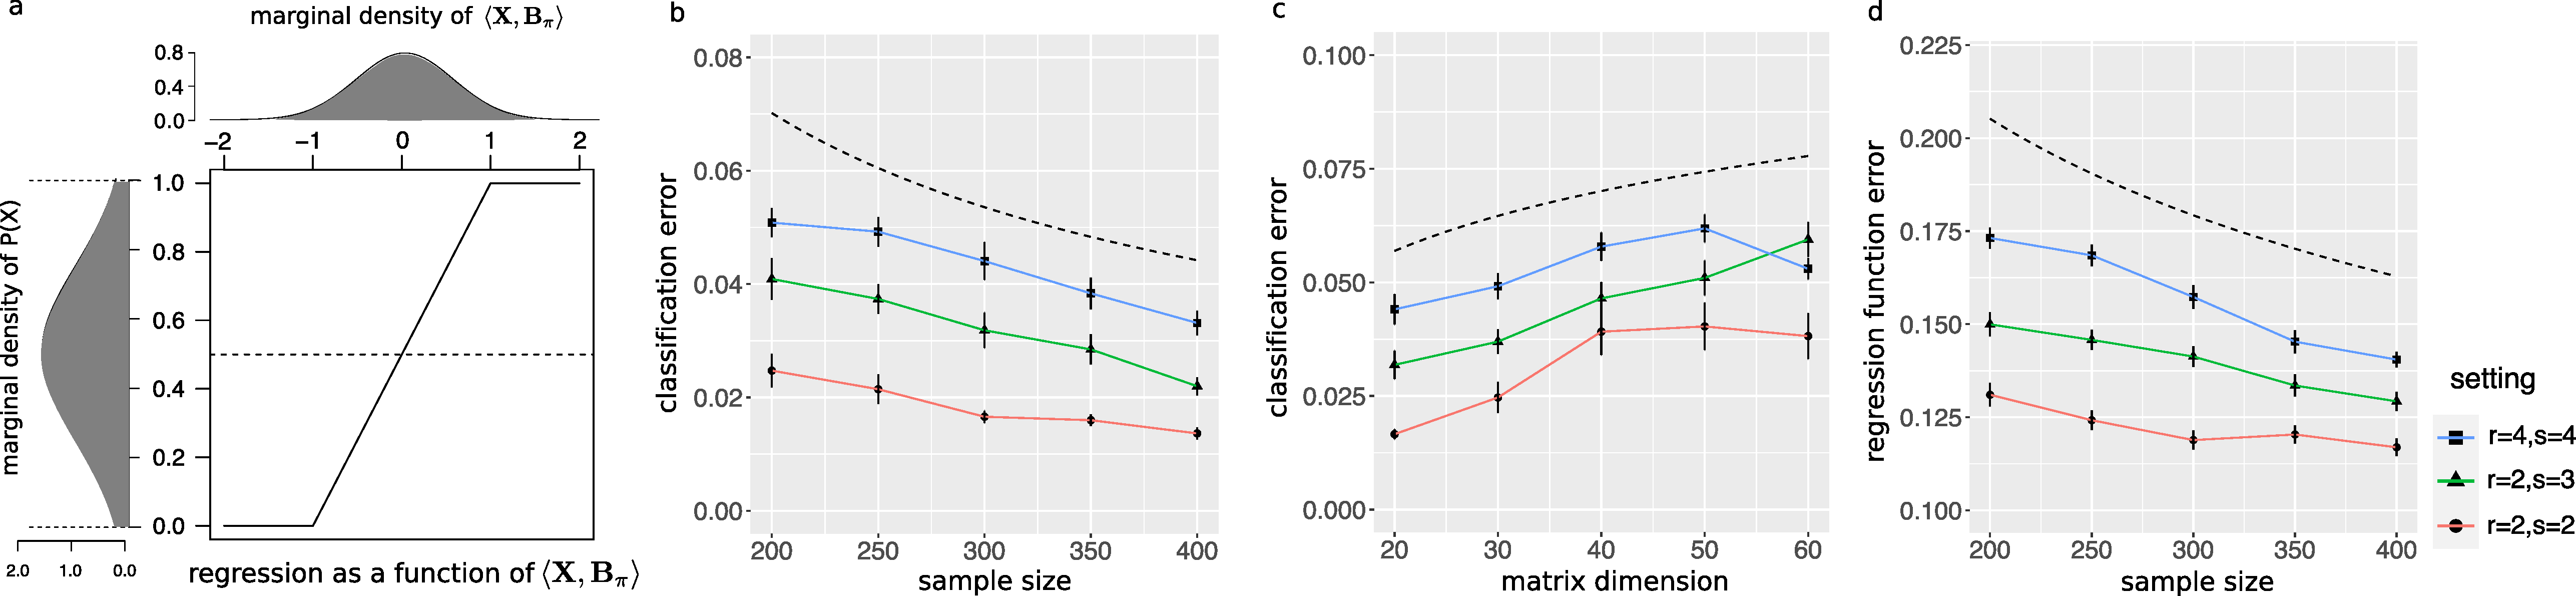
\includegraphics[width=16cm]{combined_linear.pdf}
    \caption{Finite sample accuracy of matrix classification and regression. (a) simulation setup. (b) classification error with sample size when $d=30$. (c) classification error with matrix dimension when $n=200$. (d) regression error with sample size. 
    The dash line in panels (b)-(d) represent theoretical rate $\tO(n^{-2/3})$, $\tO(\log d)$, and $\tO(n^{-1/3})$, respectively. }\label{fig:linear}
\end{figure}

\begin{figure}[ht]
    \centering
   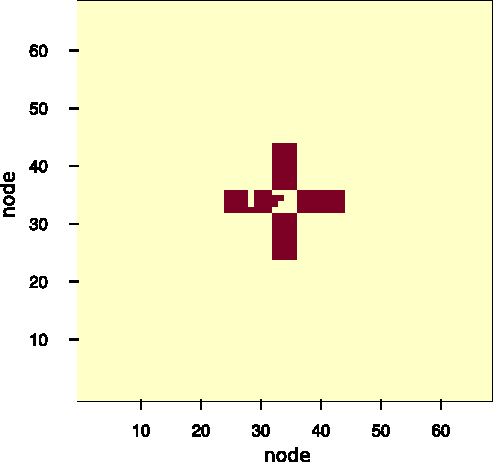
\includegraphics[width=3.7cm]{est_cross.pdf}
      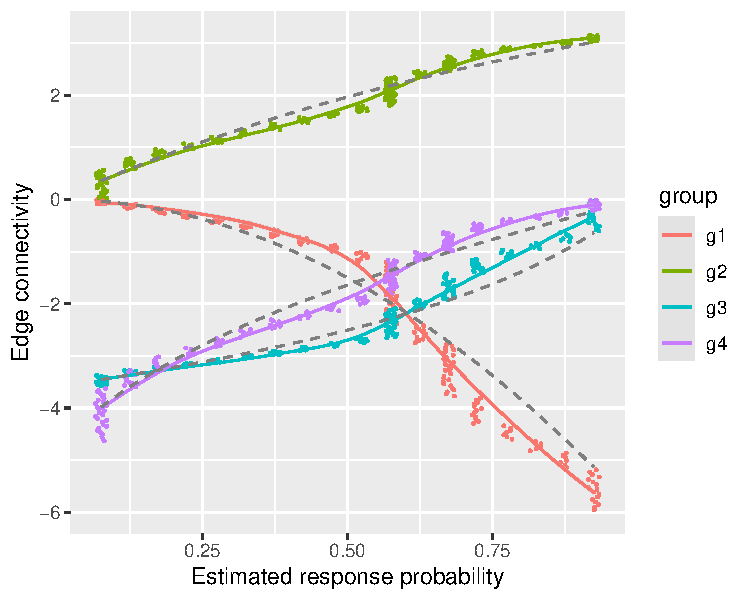
\includegraphics[width=4.3cm]{FMD_cross.pdf}
          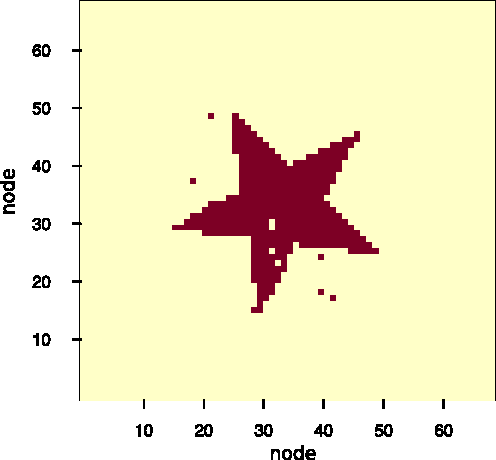
\includegraphics[width=3.7cm]{est_star.pdf}
               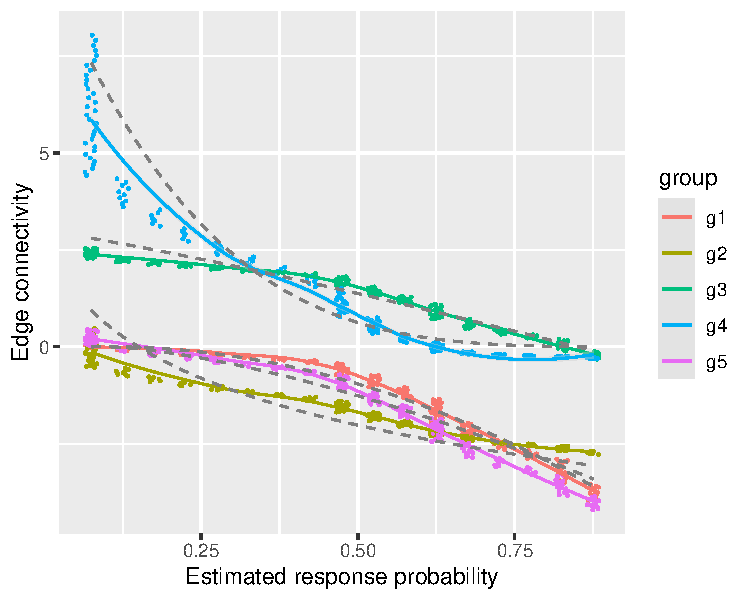
\includegraphics[width=4.3cm]{FMD_star.pdf}
 \caption{Example outputs returned by {\bf \small NonMAR}. Panels (a) and (c) plot the top edges selected by our method. Panels (b) and (d) are scatter plots of the edge connectivity strength (averaged by subregion) versus the estimated response probability. The ground truth function is depicted in dashed curve.}\label{fig:compare3}
\end{figure}


\clearpage
\subsection{Proofs}
\subsubsection{Proof of Proposition~\ref{thm:identifiability}}
\begin{proof}[Proof of Proposition~\ref{thm:identifiability}]
For ease of notation, we drop the argument $\pi$ from $S_{\text{bayes}}(\pi)$, $R_\pi(\cdot)$, and $d_\pi(\cdot,\cdot)$, and simply write $S_{\text{bayes}}$, $R(\cdot)$, and $d(\cdot,\cdot)$ respectively. The following identity is useful to relate the excess risk and set difference in classifiers,
\begin{align}\label{eq:excess}
d(S,\bayesS) &\stackrel{\text{def}}{=} R(S)-R(\bayesS)\\
& = \mathbb{E}_{\mX,y}\left[w(y)\mathds{1}(y\neq I(S))\right]-\mathbb{E}_{\mX,y}\left[w(y)\mathds{1}(y\neq I(\bayesS))\right]\notag \\
&=\mathbb{E}_{\mX}\left[(\pi-\mu(\mX))\left(I(S)-I(\bayesS)\right)\right]\notag \\
&=2\int_{\mX\in S\Delta S_{\text{bayes}}}|\mu(\mX)-\pi|d \mathbb{P}_{\mX}.
\end{align}

We divide the proof into two cases: $\alpha \in (0,1)$ and $\alpha=1$. 
\begin{enumerate}[label={2.\arabic*},wide, labelwidth=!, labelindent=0pt]
\item[Case 1:] $\alpha \in (0,1)$.

Consider an arbitrary set $S\subset\mathbb{R}^{d_1\times d_2}$. Let $t$ be an arbitrary number in the interval $[0,1]$, and define the set $A=\{\mX\colon |\mu(\mX)-\pi|>t\}$. 
\begin{align}
\int_{\mX\in S\Delta S_{\text{bayes}}}|\mu(\mX)-\pi|d \mathbb{P}_{\mX} &\geq t \left[\mathbb{P}_{\mX}(\left(S\Delta S_{\text{bayes}}) \cap A\right)\right] \\
&\geq t\left( \mathbb{P}_{\mX}\left(S\Delta S_{\text{bayes}}\right) - \mathbb{P}_{\mX}(A^c)\right)\\
&\geq t\left( \mathbb{P}_{\mX}\left(S\Delta S_{\text{bayes}}\right) - Ct^{\alpha\over 1-\alpha}\right),\quad \text{for all }0\leq t < \rho(\pi,\tN).
\end{align}
Combining the above inequality with the identity~\eqref{eq:excess} yields
\begin{equation}\label{eq:tail2}
d(S,\bayesS)\geq 2t\left( \mathbb{P}_{\mX}\left(S\Delta S_{\text{bayes}}\right) - Ct^{\alpha\over 1-\alpha}\right),\quad \text{for all }t\in(0,\rho(\pi,\tN)]).
\end{equation}
We maximize the lower bound of~\eqref{eq:tail2} with respect to $t$ and obtain the optimal $0\leq t_{\text{opt}}<\rho(\pi,\tN)$,
\[
t_{\text{opt}}=\begin{cases}
\rho(\pi,\tN), & \text{if}\quad \mathbb{P}_{\mX}\left(S\Delta S_{\text{bayes}}\right)\geq {C\over 1-\alpha}\rho(\pi,\tN)^{{\alpha\over1-\alpha}} ,\\
\left[{1-\alpha \over C}\mathbb{P}_{\mX}\left(S\Delta S_{\text{bayes}}\right)\right]^{1-\alpha \over \alpha}, & \text{if}\quad \mathbb{P}_{\mX}\left(S\Delta S_{\text{bayes}}\right)< {C\over 1-\alpha} \rho(\pi,\tN)^{{\alpha\over1-\alpha}}.
\end{cases}
\]
The corresponding lower bound of the inequality~\eqref{eq:tail2} becomes
\begin{align}
  d(S,\bayesS)\geq\begin{cases}
2\alpha\rho(\pi,\tN)\mathbb{P}_{\mX}(S\Delta \bayesS), & \text{if}\quad \mathbb{P}_{\mX}\left(S\Delta S_{\text{bayes}}\right)\geq {C\over 1-\alpha}\rho(\pi,\tN)^{{\alpha\over1-\alpha}} ,\\
2\alpha{\left(1-\alpha\over C\right)}^{1-\alpha \over \alpha} \mathbb{P}^{1\over \alpha}_{\mX}\left(S\Delta S_{\text{bayes}}\right), & \text{if}\quad \mathbb{P}_{\mX}\left(S\Delta S_{\text{bayes}}\right)< {C\over 1-\alpha} \rho(\pi,\tN)^{{\alpha\over1-\alpha}}.
\end{cases}
\end{align}

Combining both cases gives
\begin{align}\label{eq:cmultiidentity}
    d_\Delta(S,\bayesS) \stackrel{\text{def}}{=}\mathbb{P}(S\Delta\bayesS)\leq c\left(d^\alpha(S,\bayesS)+\frac{1}{\rho(\pi,\tN)}d(S,\bayesS)\right),
\end{align}

where we take $c= \max\left(\frac{1}{2\alpha},\left(C\over 1-\alpha\right)^{1-\alpha}\left(1\over 2\alpha\right)^\alpha\right)$. 

\item [Case 2:] $\alpha = 1$.

The inequality~\eqref{eq:tail2} now becomes
\[
d(S,\bayesS)\geq 2t\mathbb{P}_{\mX}(S\Delta \bayesS) = 2td_\Delta(S,\bayesS), \quad \text{for all }0\leq t < \rho(\pi,\tN).
\]
The conclusion \eqref{eq:cmultiidentity} follows by taking $t=1/\rho(\pi,\tN)$ into the above inequality.
\end{enumerate}
Therefore,  Proposition~\ref{thm:identifiability} holds.
\end{proof}



\subsubsection{Proof of Theorem~\ref{thm:twobounds}}
\begin{proof}[Proof of Theorem~\ref{thm:twobounds}]
It follows from the definition of $\bar \mu(\mX)$ that
\begin{align}
|\mu(\mX)-\bar \mu(\mX)| &\leq {1\over 2H}\sum_{\pi \in \Pi}\left|I(\mX\in \bar S(\pi)) -I(\mX\in \bayesS(\pi))\right| + \big|\mu(\mX) - {1\over 2}-{1\over 2H}\sum_{\pi \in \Pi}I(\mX\in \bayesS(\pi))\big|\\
&= {1\over H}\sum_{\pi \in \Pi}\mathds{1}(\mX \in \bar S(\pi) \Delta \bayesS(\pi))+\left| \mu(\mX)-  {1\over 2H}\left(1+2\sum_{\pi \in \Pi}\mathds{1}(\mX \in \bayesS(\pi))\right) \right|\\
&\leq  {1\over H}\sum_{\pi \in \Pi}\mathds{1}(\mX \in \bar S(\pi) \Delta \bayesS(\pi))+ {1\over 2H}\\&\leq\frac{1}{H}\sum_{\pi\in\Pi\setminus\tN}\mathds{1}(\mX \in \bar S(\pi) \Delta \bayesS(\pi))+ {1+2c\over 2H},
\end{align}
where the last inequality follows from the assumption that $|\tN|\leq c$.
Taking expectation with respect to $\mX$ on both sides gives
\begin{align}
\mathbb{E}|\mu(\mX)-\bar \mu(\mX)|&\leq \frac{1}{H}\sum_{\pi\in\Pi\setminus\tN}d_\Delta(\bar S(\pi), \bayesS(\pi))+{1+2c\over 2H}\\&\lesssim \frac{1}{H}\sum_{\pi\in\Pi\setminus\tN}\left[d_\pi^\alpha(\bar S(\pi), \bayesS(\pi))+\frac{1}{\rho(\pi,\tN)}d_\pi(\bar S(\pi), \bayesS(\pi))\right]+{1\over H},
\end{align}
where the last line comes from Proposition~\ref{thm:identifiability}. 
Furthermore, the definition of regression risk~\eqref{eq:regression} implies
\begin{align}
R_\text{reg}(\bar \mu)-R_\text{reg}(p)&=\mathbb{E}_{(\mX,y)}\left(|2\bar \mu(\mX)-y-1|^2-|2\mu(\mX)-y-1|^2\right)\\
&= 4\mathbb{E}_{\mX}\left[p^2(\mX)+\bar \mu^2(\mX)-2\mu(\mX)\bar \mu(\mX)\right]\\
&=4\mathbb{E}_{\mX}[\mu(\mX)-\bar \mu(\mX)]^2\\
&\leq 4\mathbb{E}_{\mX}|\mu(\mX)-\bar \mu(\mX)|.
\end{align}
\end{proof}

\subsubsection{Proof of Proposition~\ref{prop:polynomial}}\label{sec:population}
\begin{prop}[Polynomial continuity of inverse links]\label{prop:polynomial}
Consider the parametric model $p=g\circ f$ as in Example 1, where we assume random predictors $\mX$ with i.i.d.\ Uniform$[0,1]$ entries. Suppose the inverse link function has a constant $c_1,c_2>0$ and $\alpha\in[0,1]$ such that  $g^{-1}(\pi+t)-g^{-1}(\pi-t) \leq c_1 t^{\alpha\over 1-\alpha}$ for all $t\in[0,c_2)$. Then,
\begin{equation}\label{eq:concentration}
\mathbb{P}(|\mu(\mX)-\pi|\leq t)\leq c_3t^{\alpha\over 1-\alpha}, \quad \text{for all  }t\in[0,c_2),
\end{equation}
where $c_3>0$ is a constant depending on $\pi\in(0,1)$. In particular, when the function $g$ is the identity or logistic link, we have $\alpha=1/2$.
\end{prop}
\begin{proof}
 Let $f(\mx) = \langle \mb,\mx\rangle$ where $\mb = (b_1,\ldots, b_d)\in\mathbb{R}^{d}$ and $\mx = (x_1,\ldots,x_d)\in[0,1]^d.$
First we prove that 
\begin{align}\label{eq:mainineq}
    \int_{\{\mx: l(t)\leq \langle \mb,\mx\rangle \leq u(t)\}}d\mx \leq c_d t^{\alpha\over 1-\alpha}
\end{align} for any $l(t)$ and $u(t)$ such that $u(t)-l(t)  \leq c t^{\alpha\over 1-\alpha}$ for some constant $c>0.$

\begin{enumerate}
    \item Consider the case when $d = 1$ where $\mx = x_1 \in [0,1]$ and $\mb = b_1\in \mathbb{R}$.
    \begin{align}
        \int_{\{\mx:l(t)\leq \langle \mb,\mx\rangle \leq u(t)\}}d\mx = \int_{\frac{l(t)}{b_1}\leq x_1 \leq\frac{u(t)}{b_1}}dx_1 \leq c_1t^{\alpha\over 1-\alpha}.
    \end{align}
    \item Suppose that when $d = k$ where $\mx = (x_1,\ldots,x_k)\in[0,1]^k$ and $\mb = (b_1,\ldots,b_k)\in\mathbb{R}^k$, the following is satisfied.
    \begin{align}
        \int_{\{\mx:l(t)\leq \langle\mb,\mx\rangle\leq u(t)\}} d\mx \leq c_k t^{\alpha\over 1-\alpha}.
    \end{align} 
    \item Consider the case when $d = k+1$ where $\mx = (x_1,\ldots,x_{k+1})\in[0,1]^{k+1}$ and $\mb = (b_1,\ldots,b_{k+1})\in\mathbb{R}^{k+1}$.
   
    \begin{align}
        \int_{\{\mx:l(t)\leq \langle \mb,\mx\rangle \leq u(t)\}} d\mx  &= \int_{\{\mx:l(t)-b_{k+1}x_{k+1}\leq b_1x_1+\ldots b_kx_k\leq u(t)-b_{k+1}x_{k+1}\}} d\mx_{1:k}dx_{k+1} \\&\leq \int_{0}^{1}\int_{l(t)-b_{k+1}x_{k+1}\leq b_1x_1+\ldots b_kx_k\leq u(t)-b_{k+1}x_{k+1}}\,d\mx_{1:k}dx_{k+1}\\&\leq \int_{0}^1 c_kt^{\alpha\over 1-\alpha}\,dx_{k+1} \\&\leq c_{k+1}t^{\alpha\over 1-\alpha}.
    \end{align}
    \item By mathematical induction, \eqref{eq:mainineq} holds for arbitrary $d.$
 \end{enumerate}
 Notice that
 \begin{align}
     \mathbb{P}(|\mu(\mX)-\pi|\leq t) &= \mathbb{P}(\pi-t \leq \mu(\mX)\leq \pi+t)\\&= \mathbb{P}(\pi-t\leq g(\langle \mB,\mX\rangle )\leq \pi+t)\\&=\mathbb{P}(g^{-1}(\pi-t)\leq \langle\mB,\mX\rangle\leq g^{-1}(\pi+t)).
 \end{align}
Combining  the assumption that $g^{-1}(\pi+t)-g^{-1}(\pi-t) \leq c_1t^{\alpha\over 1-\alpha}$ for all $t\in[0,c_2)$ and \eqref{eq:mainineq} gives
 \begin{align}
     \mathbb{P}(|\mu(\mX)-\pi|\leq t/H)\leq c_3 t^{\alpha\over 1-\alpha},  \text{ for all } t\in[0,c_2).
 \end{align}
 
 In particular, when the link function is the identity or logistic link we have $\alpha = 1/2$.
 
 
 When $g(z) = z$, we have 
 \begin{align}
     g^{-1}(\pi+t)-g^{-1}(\pi-t) = 2t.
 \end{align}


 When $g(z) = \frac{e^z}{1+e^z}$, we have 
 \begin{align}
      g^{-1}(\pi+t)-g^{-1}(\pi-t) &=\log\left(\pi-t\over1-(\pi-t)\right)-\log\left(\pi+t\over1-(\pi+t)\right)\\&=\frac{2}{\pi^*(1-\pi^*)}t,
 \end{align}
 for some $\pi^*\in[\pi-t,\pi+t]$ by mean value theorem.
 
 Therefore, we have $\alpha = 1/2$ when the link function is the identity or logistic link.
 \end{proof}


\subsubsection{Proof of Theorem~\ref{thm:main}}
\begin{proof}[Proof of Theorem~\ref{thm:main}]
Our proof adopts the techniques of~\citet[Theorem 3]{wang2008probability} to the contexts of classifier functions $\tF(r,s_1,s_2)$. We summarize only the key difference here but refer to~\cite{wang2008probability} for complete proof. 

Let $\hat f = I(\hat S_{\text{bayes}}(\pi)),\bayesf = I(\bayesS(\pi))$ be the indicator functions corresponding to the set $\hat S_{\text{bayes}}(\pi),\bayesS(\pi)\subset \mathbb{R}^{d_1\times d_2}$, respectively .
From Proposition~\ref{prop:equivalance},  $(\pi,\alpha)$-local regularity implies 
\begin{align}
\text{Var}[w(y)\ell(yf(\mX))-w(y)\ell(y\bayespif(\mX))]\lesssim [R_{\ell,\pi}(f)-R_{\ell,\pi}(\bayespif)]^\alpha.
\end{align}
Notice $\rho(\pi,\tN)$ is a constant in the proposition because we only consider a given $\pi$.
Applying the second order condition to Theorem 3 of \cite{wang2008probability} gives that, with the choice $\lambda\leq {t_n\over 4J_n}$, 
\begin{equation}\label{eq:rate}
\mathbb{P}\left[R_{\ell,\pi}(\hat f)-R_{\ell,\pi}(\bayesf)\geq \max\left\{a_n, t_n\right\}\right]\leq {7\over 2}\exp\left( -Cn(\lambda J_n)^{2-\alpha}\right), 
\end{equation}
where $C>0$. Here $\{a_n\}$ is the vanishing sequence specified in~Assumption~\ref{ass:main}. Combining \eqref{eq:excess-hinge} and \eqref{eq:rate} gives
\begin{equation}
\mathbb{P}\left[d_\pi\left(\hat S_{\text{bayes}}(\pi),\bayesS(\pi)\right)\geq \max\left\{a_n, t_n\right\}\right]\leq {7\over 2}\exp\left( -Cn(\lambda J_n)^{2-\alpha}\right).
\end{equation}
The rate of convergence $t_n>0$ is determined by the solution to the following inequality,
\begin{equation}\label{eq:equation}
\sup_{k\geq 2}{1\over L}\int_{L}^{L^{\alpha/2}}\sqrt{\tH_{[\ ]}(\varepsilon, \tF^{k},\vnormSize{}{\cdot})}d\varepsilon \leq n^{1/2}, \quad \text{where }L=t_n+\lambda J_n(k/2-1).
\end{equation}
In particular, the smallest $t_n$ satisfying~\eqref{eq:equation} yields the best upper bound of the error rate. Here $\tH_{[\ ]}(\varepsilon, \tF^{k}, \vnormSize{}{\cdot})$ denotes the $L_2$-norm, $\varepsilon$-bracketing number for function family $\tF^{k}$, and for all $k\in \mathbb{N}_{+}$, we define $\tF^{k}=\{f\in\tF(r,s_1,s_2)\colon \FnormSize{}{f}^2\leq k\}$; i.e., the subset of functions in $\tF(r,s_1,s_2)$ with magnitudes bounded by $k$. 

It remains to solve for the smallest possible $t_n$ in~\eqref{eq:equation}. Based on Lemma~\ref{lem:metric}, the inequality~\eqref{eq:equation} is satisfied with 
\begin{equation}\label{eq:delta}
t_n\asymp  \left({r(s_1+s_2)\log d \over n}\right)^{1/(2-\alpha)} \quad \text{and}\quad \lambda \asymp {t_n\over J_n},
\end{equation}
Plugging~\eqref{eq:delta} into~\eqref{eq:rate} gives
\begin{align}\label{eq:tail}
\mathbb{P}\left[d_\pi\left(\hat S_{\text{bayes}}(\pi),\bayesS(\pi)\right)\geq  \max\left\{ a_n, C_1\left({r(s_1+s_2)\log d \over n}\right)^{1/(2-\alpha)} \right\}\right]&\leq {7\over 2}\exp\left( - C_2r(s_1+s_2)\log d \right)\notag \\
&\leq d^{-C_3r(s_1+s_2)},
\end{align}
where $C_1, C_2, C_3>0$ are constants.
\end{proof}


\subsubsection{Proofs of Theorem~\ref{thm:regression}}
We first suggest lemmas and proposition that will be used to prove Theorem~\ref{thm:regression}.
\begin{lem}[Multiple level-sets estimation]~\label{lem:main}Suppose $\mu(\mX)$ is $\alpha$-globally regular with $\alpha\in[0,1]$. Denote $t_n={ r(s_1+s_2)\log d  \over n}$ for $n\in\mathbb{N}_{+}$. Then, under the same condition and high probability specified in Theorem~\ref{thm:main}, we have
\[
d_{\Delta}(\bayesS(\pi),\hat S(\pi))\lesssim t_n^{\alpha/(2-\alpha)}+ {1\over \rho^2(\pi,\tN)}t_n,\quad \text{for all levels }\pi \notin \tN, 
\]
 Furthermore, 
\begin{equation}\label{eq:total}
{1\over H}\sum_{\pi \in \Pi} d_{\Delta}(\bayesS(\pi),\hat S(\pi))\lesssim   {1\over H}+t_n^{\alpha/(2-\alpha)}+ H t_n .
\end{equation}
\end{lem}

\begin{proof}[Proof of Lemma~\ref{lem:main}] The $\alpha$-global regularity of $\mu(\mX)$ implies that, for all $\pi \notin \tN$, the conversion inequality holds by Proposition~\ref{prop:equivalance},
\begin{equation}\label{eq:conversion2}
d_{\Delta}(\bayesS(\pi),S) \lesssim
\begin{cases}
d^\alpha_{\pi}(\bayesS(\pi),S), & \text{if }S\in \textup{I},\\
{1\over \rho(\pi, \tN)}d_{\pi}(\bayesS,S),& \text{otherwise},
\end{cases}
\end{equation}
where region  $\textup{I}=\{S \colon d_{\Delta}(\bayesS(\pi),S)\leq \frac	{C}{1-\alpha}\rho(\pi,\tN)^{\alpha/(1-\alpha)}\}$.
In addition,  the mean-to-variance inequality also holds by Proposition~\ref{prop:equivalance},
\begin{equation}
%\text{Var}\left[w(y)\ell(f(\mX)) - w(y)\ell(\bayesf(\mX))\right]  \leq
%\begin{cases} 
%\left[R_{\ell,\pi}(f)-R_{\ell,\pi}(\bayesf)\right]^{\alpha},& \text{if }\{\mX\colon f(\mX)\geq 0\}\in\textup{I},\\
% {1\over \rho(\pi, \tN)}\left[R_{\ell,\pi}(f)-R_{\ell,\pi}(\bayesf)\right],& \text{otherwise}.
%\end{cases}
\text{Var}\left[w(y)\ell(f(\mX)) - w(y)\ell(\bayesf(\mX))\right] \lesssim \left[R_{\ell,\pi}(f)-R_{\ell,\pi}(\bayesf)\right]^{\alpha}+ {1\over \rho(\pi, \tN)}\left[R_{\ell,\pi}(f)-R_{\ell,\pi}(\bayesf)\right].
\end{equation}
Applying Theorem~\ref{thm:main} and Lemma~\ref{lem:metric} to the above mean-to-variance relationship, we obtain the classification risk bound,
\begin{align}
d_\pi(\bayesS(\pi), \hat S(\pi))\lesssim t_n^{1/(2-\alpha)}+ {1\over \rho(\pi, \tN)}t_n,\quad \text{where}\ t_n={r(s_1+s_2)\log d  \over n}.
\end{align}
Plugging the above bound into~\eqref{eq:conversion2}, we obtain
\begin{align}
d_{\Delta}(\bayesS(\pi),\hat S(\pi)) &\lesssim d^\alpha_{\pi}(\bayesS(\pi),S)+{1\over \rho(\pi, \tN)}d_{\pi}(\bayesS(\pi),S)\\
&\lesssim t_n^{\alpha/(2-\alpha)}+{1\over \rho^{\alpha}(\pi, \tN)}t_n^{\alpha}+{1\over \rho(\pi, \tN)}t_n^{1/(2-\alpha)}+{1\over \rho^2(\pi, \tN)}t_n\\
%&\leq {t_n\over \rho^2(\pi, \tN)}\left( \rho^2{\pi, \tN}          \right)
%&\leq t^{\alpha/(2-\alpha)}_n\left(1+{1\over \rho(\pi, \tN)}t_n^{(1-\alpha)/(2-\alpha)}\right)^\alpha+{t^{1/(2-\alpha)}_n\over \rho(\pi, \tN)}\left(1+{1\over \rho(\pi, \tN)}t_n^{(1-\alpha)/(2-\alpha)}\right)\\
&\leq 4t_n^{\alpha/(2-\alpha)}+{4\over \rho^2(\pi, \tN)}t_n.
\end{align}
where the last line follows from the fact that $a(b^2+b^{2-\alpha}+b+1) \leq 4 a (b^2+1)$ with $a:={t_n \over \rho^2(\pi, \tN)}$ and $b:=\rho(\pi, \tN) t_n^{(\alpha-1)/(2-\alpha)}$.  Therefore,  we obtain the first conclusion.


To prove the second conclusion~\eqref{eq:total}, we write 
\begin{align}\label{eq:twobounds}
{1\over H}\sum_{\pi \in \Pi} d_{\Delta}(\bayesS(\pi),\hat S(\pi))={1\over H}\sum_{\pi \in \Pi\cap \tN_H} d_{\Delta}(\bayesS(\pi),\hat S(\pi))+{1\over H}\sum_{\pi \in \Pi\cap \tN_H^c} d_{\Delta}(\bayesS(\pi),\hat S(\pi)),
\end{align}
where $\tN_H \stackrel{\text{def}}{=}\bigcup_{\pi'\in\tN}\left(\pi'-\frac{1}{H},\pi'+\frac{1}{H}\right)$.
The first term involves only finite number of summands and thus can be bounded by $2c/H$ where $c>0$ is a constant such that $|\tN|\leq c$.  We bound the second term using the explicit forms of $\rho(\pi, \tN)$ in the sequence $\pi \in\Pi\cap \tN_H^c$,
\begin{align}
{1\over H}\sum_{\pi \in \Pi\cap \tN_H^c} d_{\Delta,}(\bayesS(\pi),\hat S(\pi)) &\lesssim  {1\over H}\sum_{\pi\in \Pi\cap \tN_H^c} t_n^{\alpha/(2-\alpha)}+{t_n\over H}\sum_{\pi \in \Pi\cap \tN_H^c}{1\over \rho^2(\pi, \tN)}\\
&\leq t_n^{\alpha/(2-\alpha)}+{t_n\over H} \sum_{\pi \in \Pi\cap \tN_H^c} \sum_{\pi' \in \tN}{1\over |\pi-\pi'|^2}\\
&\leq  t_n^{\alpha/(2-\alpha)}+{t_n\over H} \sum_{\pi'\in \tN} \sum_{\pi \in \Pi\cap \tN_H^c}{1\over |\pi-\pi'|^2}\\
&\leq t_n^{\alpha/(2-\alpha)}+ {t_n\over H} \sum_{\pi'\in \tN} 2H^2\\
&\leq t_n^{\alpha/(2-\alpha)}+ 2cHt_n,
\end{align}
where the last inequality follows from the Lemma~\ref{lem:H}.  Combining the bounds for the last two terms in \eqref{eq:twobounds} completes the second conclusion.  As seen from the calculation, the distance $\rho^2(\pi, \tN)$ grows quadratically as the level $\pi$ moves away from the mass points in $\tN$. This leads to a fast linear rate in terms of $H$, provided that there are finitely many mass points in $\tN$.
\end{proof}

\begin{lem}\label{lem:H}
Fix a $\pi'\in\tN$ and a sequence $\Pi=\{1/H,\ldots,(H-1)/H\}$ with $H\geq 2$. Then, 
\[
\sum_{\pi \in \Pi\cap \tN_H^c}{1\over 
|\pi-\pi'|^2}\leq 2H^2. 
\]
\begin{proof}
Notice that  all points $\pi\in\Pi\cap\tN_H^c$ satisfy 
$|\pi-\pi'|>{1\over H}$ for all $\pi'\in\tN$.
\begin{align}
   \sum_{\pi \in \Pi\cap \tN_H^c}{1\over |\pi-\pi'|^2}&= \sum_{\frac{h}{H}\in\Pi\cap \tN_H^c } {1\over |\frac{h}{H}-\pi'|^2}\\
   &\leq H^2 \sum_{h=1}^{H}{1 \over h^2}\\
 &\leq H^2\left\{ 1+\int_{1}^2{1\over x^2}dx+ \int_{2}^3{1\over x^2}dx+\cdots + \int_{H-1}^H{1\over x^2}dx\right\}\\
&= H^2\left(1+\int^{H}_{1}{1\over x^2}dx\right) \leq 2H^2,
\end{align}
 where the third line uses the monotonicity of ${1\over x^2}$ for $x\geq 1$. 
 \end{proof}
\end{lem}

\begin{prop}\label{prop:equivalance}
Let $\pi\in(0,1)$ denote a given level value, and $R_{\ell,\pi}(f)=\mathbb{E}[w(y)\ell(yf(\mX))]$ denote the weighted hinge risk  or $\psi$ risk for the decision function $f$. Suppose Definition~\ref{ass:decboundary}
holds with $\alpha\in(0,1]$ and $C>0$. Then, the following two properties hold for bounded functions $f\in\tF(r,s_1,s_2)$. 
\begin{enumerate}
\item Conversion inequality:  
\begin{equation}\label{eq:conversion}
d_{\Delta}(\bayesS(\pi),S) \lesssim
\begin{cases}
d^\alpha_{\pi}(\bayesS(\pi),S), & \text{if }S\in \textup{I},\\
{1\over \rho(\pi, \tN)}d_{\pi}(\bayesS(\pi),S),& \text{otherwise},
\end{cases}
\end{equation}
where the region $\textup{I}=\{S \colon d_{\Delta}(\bayesS(\pi),S)\leq \frac	{C}{1-\alpha}\rho(\pi,\tN)^{\alpha/(1-\alpha)}\}$.
\item Mean-variance relationship:
\begin{equation}
\text{Var}\left[w(y)\ell(f(\mX)) - w(y)\ell(\bayesf(\mX))\right]  \lesssim 
\left[R_{\ell,\pi}(f)-R_{\ell,\pi}(\bayesf)\right]^{\alpha}+
 {1\over \rho(\pi, \tN)}\left[R_{\ell,\pi}(f)-R_{\ell,\pi}(\bayesf)\right].
\end{equation}
\end{enumerate}
\end{prop}

\begin{proof}
Property 1 follows directly from the proof in Proposition~\ref{thm:identifiability}.
For Property 2, we devide the proof into two cases: when $\ell(\cdot)$ is hinge loss and  $\psi$ loss. 

\begin{enumerate}[label={2.\arabic*},wide, labelwidth=!, labelindent=0pt]
\item[Case 1:] When $\ell(z) = (1-z)_+$.

Property 2 follows from Lemma~\ref{lem:hingeL1} and the boundedness of $f$. Specifically, we bound the variance using the $L$-1 distance between $f$ and $\bayespif$, 
\begin{align}
\text{Var}[w(y)\ell(yf(\mX))-w(y)\ell(y\bayespif(\mX))]&\leq  L\mathbb{E}|\ell(yf(\mX))-\ell(y\bayespif(\mX))|\\
&\leq L\mathbb{E}|f(\mX)-\bayespif(\mX)|
\end{align}
where $L>0$ is a constant that bounds the magnitude of $f$ in the local neighborhood of $R_{\ell,\pi}(\bayespif)$ (c.f. Assumption~\ref{ass:main}), the second line comes form the Lipschitz continuity of the hinge loss.  Applying  Lemma~\ref{lem:hingeL1} on the last inequality complete the proof.

\item[Case 2:] When $\ell(z) = 2\min(1,(1-z)_+)$.
Notice that 
\begin{align}
\text{Var}\left[w(y)\ell(yf(\mX))-w(y)\ell(y\bayesf(\mX))\right]
\leq & \mathbb{E}|w(y)\ell(yf(\mX))-w(y)\ell(y\bayespif(\mX))|^2\\
\leq& \ L\mathbb{E}|w(y)\ell(yf(\mX))-w(y)\ell(y\bayespif(\mX))|\\
\leq &\ L\KeepStyleUnderBrace{\mathbb{E}\left| w(y)\left(1-\sign(yf(\mX))\right)- w(y)\ell(y\bayespif(\mX))\right
|}_{=:\text{(i)}}\\&+L\KeepStyleUnderBrace{\mathbb{E}\left| w(y)\ell(yf(\mX))- w(y)\left(1-\sign(yf(\mX))\right) \right|}_{=:\text{(ii)}},
\end{align}
(i) is bounded as follows
\begin{align}
\text{(i)}=\mathbb{E}\left[w(y)\left|\sign (yf(\mX))-\sign (y\bayesf(\mX))\right|\right]&\leq 2d_\Delta(\bayesS(\pi),S)\\&\lesssim  d^\alpha_{\pi}(\bayesS(\pi),S)+{1\over \rho(\pi, \tN)}d_{\pi}(\bayesS(\pi),S),
\end{align}
where the last inequality is from Property 1.
(ii) bounded as follows
\begin{align}
    \text{(ii)}
    &=\mathbb{E}\left [w(y)\ell(yf(\mX))- w(y)\left(1-\sign(yf(\mX))\right) \right]\\
    &= \mathbb{E}\left[w(y)\ell(yf(\mX))-w(y)\ell(y\bayespif(\mX))\right]+ \mathbb{E}\left[w(y)(\sign(f(\mX))-\sign(\bayespif(\mX))\right]\\&\leq [R_{\ell,\pi}(f)-R_{\ell,\pi}(\bayesf)]+2d_\Delta(\bayesS(\pi),S)\\&\lesssim  [R_{\ell,\pi}(f)-R_{\ell,\pi}(\bayesf)]+ d^\alpha_{\pi}(\bayesS(\pi),S)+{1\over \rho(\pi, \tN)}d_{\pi}(\bayesS(\pi),S),
\end{align}
where the last inequality is form Property 1.
Combining \eqref{eq:excess-hinge} and two bounds (i),(ii) completes the proof.
\end{enumerate}
\end{proof}

\begin{proof}[Proof of Theorem~\ref{thm:regression}]
Note that the proof of Theorem~\ref{thm:twobounds} still holds by replacing $\bar S(\pi)$ with $\hat S(\pi)$. Based on Lemma~\ref{lem:main} and Theorem~\ref{thm:main}, with $1-C_1d^{-C_2r(s_1+s_2)}$, 
\begin{align}\label{eq:levelreg}
\mathbb{E}|\mu(\mX)-\hat \mu(\mX)|\lesssim {1\over H}+\left({r(s_1+s_2)\log d \over n}\right)^{\alpha/(2-\alpha)}+H\left({r(s_1+s_2)\log d \over n}\right)+a_n,
\end{align}
where the constants have been suppressed in the asymptotical order relationship $\lesssim$. 
\end{proof}


\clearpage
\subsection{Auxiliary lemmas}


\begin{lem}[Hinge excess loss and $L$-1 distance]\label{lem:hingeL1} Consider the same set-up as in Theorem~\ref{thm:regression}. Then, the $L$-1 distance between $f$ and $\bayesf$ is bounded by their hinge excess risk; i.e,
\begin{equation}
\mathbb{E}|f(\mX)-\bayespif(\mX)|
\lesssim
\left[R_{\ell,\pi}(f)-R_{\ell,\pi}(\bayesf)\right]^{\alpha}+
 {1\over \rho(\pi, \tN)}\left[R_{\ell,\pi}(f)-R_{\ell,\pi}(\bayesf)\right].
\end{equation}
\end{lem}

\begin{proof} For ease of notation, we drop the subscript $\pi$ and simply write $\bayesf$ and $R_\ell(\bayesf)$ in place of $\bayespif$ and $R_{\ell,\pi}(\bayespif)$. We also drop the random variable $\mX$ in the function expression, and simply use $f, \bayesf$, $\mu$, to represent the decision function, Bayes rule, and the probability function, respectively. The meaning should be clear given the contexts. 

We expand the hinge excess risk using the definition of hinge loss,
\begin{align}\label{eq:function}
R_{\ell}(f)-R_{\ell}(\bayesf)&= \mathbb{E}[w(y)(1-yf)_{+}]-\mathbb{E}[w(y)(1-y\bayesf)_{+}] \notag\\
&= \int_{\mX}w(1)\mu(1-f)_{+}d\mathbb{P}_{\mX}+\int_{\mX}w(-1)(1-\mu)(1+f)_{+}d\mathbb{P}_{\mX}\notag \\
&\quad -\int_{\mX}w(1)\mu(1-\bayesf)_{+}d\mathbb{P}_{\mX}-\int_{\mX}w(-1)(1-\mu)(1+\bayesf)_{+}d\mathbb{P}_{\mX},
\end{align}
where $w(1)=1-\pi$ and $w(-1)=\pi$. 

In order to evaluate the integral, we divide the domain $\mX$ into four exclusive regions:
\begin{itemize}
\item Region I $= \{\mX\colon \mu<\pi \text{ and }f\geq -1\}$. In this region, $\bayesf=-1$, and the integrant in~\eqref{eq:function} reduces to
\begin{align}
\Phi_{\textup{I}}&:=(1-\pi)\mu(1-f)_{+}+\pi(1-\mu)(1+f)_{+}-2(1-\pi)\mu\\
&\geq (1-\pi)\mu(1-f)+\pi(1-\mu)(1+f)-2(1-\pi)\mu\\
&=(f+1)(\pi-\mu)=|f-\bayesf||\pi-\mu|.
\end{align}
\item Region II $= \{\mX\colon \mu< \pi \text{ and }f<-1\}$. In this region, $\bayesf=-1$, and the integrant in~\eqref{eq:function} reduces to
\[
\Phi_{\textup{II}}:=(1-\pi)\mu(1-f)-2(1-\pi)\mu=(-1-f)(\mu-\mu\pi )=|f-\bayesf|(1-\pi)\mu.
\]
\item Region III $=\{ \mX\colon \mu\geq \pi \text{ and }f\leq 1\}$. In this region, $\bayesf=1$, and the integrant in~\eqref{eq:function} reduces to
\begin{align}
\Phi_{\textup{III}}&:=(1-\pi)\mu(1-f)_{+}+\pi(1-\mu)(1+f)_{+}-2\pi(1-\mu)\\
&\geq (1-\pi)\mu(1-f)+\pi(1-\mu)(1+f)-2\pi(1-\mu)\\
&=(1-f)(\mu-\pi)=|f-\bayesf||\pi-\mu|
\end{align}
\item Region IV $=\{\mX\colon \mu\geq \pi \text{ and }f> 1\}$. In this region, $\bayesf=1$, and the integrant in~\eqref{eq:function} reduces to
\[
\Phi_{\textup{IV}}:=\pi(1-\mu)(1+f)-2\pi(1-\mu)=(f-1)(\pi-\mu\pi)=|f-\bayesf|(1-\mu)\pi
\]
\end{itemize}
Therefore, the integral is evaluated as
\begin{align}\label{eq:integral}
R_{\ell}(f)-R_{\ell}(\bayesf) &= \int_{\textup{I}}\Phi_{\textup{I}} d\mathbb{P}_{\mX}+\int_{\textup{II}}\Phi_{\textup{II}} d\mathbb{P}_{\mX}+\int_{\textup{III}}\Phi_{\textup{III}} d\mathbb{P}_{\mX}+\int_{\textup{IV}}\Phi_{\textup{IV}} d\mathbb{P}_{\mX}\\
&\geq \mathbb{E}|f-\bayesf||\pi-\mu|\mathds{1}(|f|\leq 1)+ \mathbb{E}|f-\bayesf|(\pi-\mu\pi)\mathds{1}(f>1)\\
& \quad +\mathbb{E}|f-\bayesf| (\mu-\mu\pi)\mathds{1}(f<-1).
\end{align}

Note that the functions $|\pi-\mu|, (\pi-\mu\pi), (\mu-\mu\pi)$ are non-negative, $[0,1]$-valued, and satisfy~\eqref{eq:prob2} by $\alpha$-global regularity (local regularity follows the same argument).  Now we use Lemma~\ref{lem:product} to bound the three terms in the last equation.  To make sure that each term has the same order in Lemma~\ref{lem:product},  we rescale the functions $|f-\bayesf|\mathds{1}(|f|\leq1),|f-\bayesf|\mathds{1}(f>1),|f-\bayesf|\mathds{1}(f<-1)$ to have expectation 1 and set upper bound of the functions as \[L = \max\left(\mnormSize{}{|f-\bayesf|\mathds{1}(|f|\leq1)},\mnormSize{}{|f-\bayesf|\mathds{1}(f>1)},\mnormSize{}{|f-\bayesf|\mathds{1}(f<-1)}\right).\]
Then,  the last inequality is bounded either Case 1 or Case 2 from Lemma~\ref{lem:product}:
\begin{enumerate}[label={2.\arabic*},wide, labelwidth=!, labelindent=0pt]
\item[Case 1:]
\begin{align}
R_\ell(f)-R_\ell(\bayesf)  &\gtrsim [\mathbb{E} |f-\bayesf|\mathds{1}(|f|\leq 1)]^{1/\alpha}+ [\mathbb{E}|f-\bayesf|\mathds{1}(f>1)]^{1/\alpha}
+[ \mathbb{E}|f-\bayesf|\mathds{1}(f<-1)]^{1/\alpha}\\
&\geq  [\mathbb{E}|f-\bayespif|]^{1/\alpha},
\end{align}

where the last inequality uses the property that $x^{1/\alpha}+y^{1/\alpha}\geq (x+y)^{1/\alpha}$ for $x,y\geq 0$ and $\alpha\in(0,1]$.
\item[Case 2:]
\begin{align}
R_\ell(f)-R_\ell(\bayesf)  &\gtrsim \rho(\pi,\tN)\left[\mathbb{E} \left(|f-\bayesf|\mathds{1}(|f|\leq 1)+|f-\bayesf|\mathds{1}(f>1)+|f-\bayesf|\mathds{1}(f<-1)\right)\right]\\
&= \rho(\pi,\tN) \mathbb{E}|f-\bayespif|.
\end{align}
\end{enumerate}
Therefore, combining two cases gives
\begin{equation}
\mathbb{E}|f(\mX)-\bayespif(\mX)|
\lesssim
\left[R_{\ell,\pi}(f)-R_{\ell,\pi}(\bayesf)\right]^{\alpha}+
 {1\over \rho(\pi, \tN)}\left[R_{\ell,\pi}(f)-R_{\ell,\pi}(\bayesf)\right].
\end{equation}
\end{proof}

\begin{lem}[Expectation of function products]\label{lem:product}Let $\mX\in \tX$ be a random variable. Let $g\colon \tX\to [0,1]$ be a function taking values on $[0,1]$ and satisfying
\begin{align}\label{eq:prob2}
\mathbb{P}[g(\mX)\leq t] \leq Ct^{\alpha/1-\alpha}, \quad \text{for all }t\in(0,\rho],
\end{align} 
for some constants $\alpha\in(0,1]$ and $ C>0$. (When $\alpha=1$, the right hand side of~\eqref{eq:prob2} is interpreted as being zero.) Then, for all nonnegative, bounded functions $f\colon \tX\to\mathbb{R}_{\geq 0}$ with $\mnormSize{}{f}\leq L$,  the following holds true,
\[
\mathbb{E}[f(\mX)g(\mX)]
\gtrsim \begin{cases}
\rho\mathbb{E}f(\mX), &\text{if}\quad{ \mathbb{E}f(\mX)\over L}\geq {C \over 1-\alpha} \rho^{\alpha/ 1-\alpha},\\
\\
 [\mathbb{E}f(\mX)]^{1/\alpha}, &\text{if}\quad{ \mathbb{E}f(\mX)\over L}< {C\over 1-\alpha} \rho^{\alpha /1-\alpha}.
\end{cases}
\]

\end{lem}
\begin{rmk} Roughly speaking, Lemma~\ref{lem:product} bounds the function $f$ by the function product $fg$ in expectation, provided that the multiplier $g$ has controlled probability mass around zero. Note that we always have the lower bound $\mathbb{E}f(\mX)g(\mX)\leq \mathbb{E}f(\mX)$ because of the boundedness of $g$. 
\end{rmk}

\begin{proof} Let $t>0$ be an arbitrary number in the interval $(0,\rho]$. We bound the expectation of the product $fg$ using the integral over the region $\{\mX\colon g(\mX)> t\}$, 
\begin{align}\label{eq:lowerbound}
\mathbb{E}[f(\mX)g(\mX)]& \geq  \mathbb{E}[f(\mX)\mathds{1}(g(\mX)>t)]\notag \\
& = t\mathbb{E}[f(\mX)-f(\mX)\mathds{1}(g(\mX)\leq t)]
\\
&\geq t\left(\mathbb{E}
f(\mX)-L\mathbb{P}[g(\mX)\leq t]\right)\notag \\
&\geq t\mathbb{E}f(\mX)-CLt^{1/1-\alpha}, \quad \text{for all }t\in(0,\rho],
\end{align}
%\fixme{Miaoyan}{the following proof needs to be updated to reflex the additional $H$..}
where the third line uses the fact that $f(\mX)\in[0,L]$, and the last line follows from~\eqref{eq:prob2}. We maximize the lower bound~\eqref{eq:lowerbound} with respect to $t\in(0,\rho]$ and obtain the optimal $t_{\text{opt}}\in(0,\rho]$,
\[
t_{\text{opt}}=\begin{cases}
\rho, & \text{if}\quad \mathbb{E}f(\mX)\geq {CL\over 1-\alpha} \rho^{\alpha/ 1-\alpha},\\
\left[{1-\alpha \over CL}\mathbb{E}f(\mX)\right]^{(1-\alpha)/ \alpha}, & \text{if}\quad \mathbb{E}f(\mX) < {CL\over 1-\alpha} \rho^{\alpha
/ 1-\alpha}.
\end{cases}
\]
The corresponding lower bound of the inequality~\eqref{eq:lowerbound} becomes
\[
\mathbb{E}[f(\mX)g(\mX)]
\geq \begin{cases}
\alpha\rho\mathbb{E}f(\mX), &\text{if}\quad \mathbb{E}f(\mX)\geq {CL \over 1-\alpha} \rho^{\alpha/ 1-\alpha},\\
\\
\alpha{\left(1-\alpha\over CL\right)}^{(1-\alpha) / \alpha} [\mathbb{E}f(\mX)]^{1/\alpha}, &\text{if}\quad \mathbb{E}f(\mX)< {CL\over 1-\alpha} \rho^{\alpha /1-\alpha}.
\end{cases}
\]
Since, $\alpha, C$, and $L$ are given constant, we have the desired results.

%\[
%\mathbb{E}[f(\mX)g(\mX)]\geq \frac{C_2}{H}\min\left\{ \mathbb{E}f(\mX),\ [\mathbb{E}f(\mX)]^{1/\alpha}\right\},
%\]
%where $C_2>0$ is a constant independent of $f$. When $\mathbb{E}f(\mX)\leq 1$, the right hand side of the above inequality takes value $C_2[\mathbb{E}(f(\mX)]^{1/\alpha}/H$. When $\mathbb{E}f(\mX)>1$, we rescale $f$ by $f/L$ and obtain
%\[
%\mathbb{E}[f(\mX)g(\mX)]\geq \frac{C_2}{H}L^{-(\alpha-1)/\alpha}[\mathbb{E}f(\mX)]^{1/\alpha}.
%\]
%Combining both cases gives the desired results. 
\end{proof}

\begin{defn}[Bracketing number]\label{pro:inftynorm}
Consider a function set $\tF$, and let $\varepsilon>0$. We call $\{(f^l_m,f^u_m)\}_{m=1}^M$ an $L_2$-metric, $\varepsilon$-bracketing function set of $\tF$, if for every $f\in \tF$, there exists an $m\in[M]$ such that 
\[
f^l_m(\mX)\leq f(\mX)\leq f^u_m(\mX),\quad \text{for all }\mX\in\mathbb{R}^{d\times d},
\]
and
\[
\vnormSize{}{f^l_m-f^u_m}\stackrel{\text{def}}{=}\sqrt{\mathbb{E}_{\mX}|f^l_m(\mX)-f^u_m(\mX)|^2} \leq \varepsilon, \ \text{for all } m=1,\ldots,M. 
\]
The bracketing number with $L_2$-metric, $\tH_{[\ ]}(\varepsilon,\ \tF,\ \vnormSize{}{\cdot})$, is defined as the logarithm of the smallest cardinality of the $\varepsilon$-bracketing function set of $\tF$.  
\end{defn}


\begin{lem}[Bracketing number for bounded functions in $\tF(r,s_1,s_2)$]\label{lem:entropy}

Let $\tF(r,s_1,s_2)$ denote the classifier functions in~\eqref{eq:class}, where we assume the intercept $b=0$ is known and that the function domain satisfies $\mathbb{P}\left(\FnormSize{}{\mX}\leq 1\right)=1$. For any given $k\in\mathbb{N}_{+}$, consider the subset of functions in $\tF(r,s_1,s_2)$ with magnitudes bounded by $k$, denoted by $\tF^k=\{f\in \tF(r,s_1,s_2)\colon \FnormSize{}{f}^2\leq k\}$. Then, there exists a constant $C>0$ such that
\[
\tH_{[\ ]}(\varepsilon,\ \tF^k,\ \vnormSize{}{\cdot}) \leq  Cr(s_1+s_2) \log {kd\over \varepsilon }.
\]
\end{lem}
\begin{proof} 
For any given $k\in\mathbb{N}_{+}$, define the matrix class
\[
\tB=\{\mB\in \mathbb{R}^{d\times d}\colon \text{rank}(\mB)\leq r,\ \text{supp}(\mB)\leq (s_1,s_2),\ \FnormSize{}{\mB}^2\leq k\}.
\]
Based on the assumption of known $b$, there is an one-to-one correspondence between functions in $\tF^k$ and matrices in $\tB$,
\[
\tF^k=\{f\colon\mX\mapsto\langle \mX,\mB\rangle+b\ \big| \ \mB\in \tB\}.
\]
Furthermore, every pair of two functions $f_1=\langle\mX, \mB_1\rangle,\ f_2=\langle \mX,\mB_2\rangle\in\tF(r,s_1,s_1)$ satisfies the norm relationship
\[
\vnormSize{}{f_1-f_2}\leq \mnormSize{}{f_1-f_2} =\sup_{\FnormSize{}{\mX}\leq 1}|\langle \mX,\mB_1\rangle -\langle \mX,\mB_2\rangle  |\leq \FnormSize{}{\mB_1-\mB_2}.
\]
Based on~\citet[Theorem 9.23]{kosorok2007introduction}, the $L_2$-metric, $(2\varepsilon)$-bracketing number in $\tF^k$ is bounded by
\[
\tH_{[\ ]}(2\varepsilon,\ \tF^k,\ \vnormSize{}{\cdot}) \leq \tH \left(\varepsilon,\ \tB,\ \FnormSize{}{\cdot}\right),
\]
where $\tH$ denotes the log covering number for the (non-bracketing) set. Therefore, it suffices to bound $\tH(\varepsilon,\ \tB,\ \FnormSize{}{\cdot})$. Now fix two subsets $S_1,S_2\subset [d]$ with $|S_1|=s_1$ and $|S_2|=s_2$, where $|\cdot|$ denotes the cardinality of the sets. Let $\tB_{S_1,S_2}\subset \tB$ denote the subset of matrices satisfying $\mB(i,j)=0$ whenever $(i,j)\notin S_1\times S_2$. Based on~\citet[Lemma 3.1]{candes2011tight}, the log covering number for $\tB_{S_1,S_2}$ is
\[
\tH \left(\varepsilon,\ \tB_{S_1,S_2},\ \Fnorm{\cdot}\right)\leq r(s_1+s_2+1)\log\left({9\sqrt{k}\over \varepsilon}\right).
\]
In view of the construction $\tB\subset\bigcup\{\tB_{S_1,S_2}\colon S_1\times S_2\subset [d_1]\times[d_2], |S_1|=s_1, |S_2|=s_2\}$, an $\varepsilon$-covering set $\tB$ is then given by the union of $\varepsilon$-covering set of $\tB_{S_1,S_2}$. Using Stirling's bound, we derive that 
\begin{align}
\tH(\varepsilon,\ \tB,\ \FnormSize{}{\cdot})&\leq \log \left\{{d \choose s_1}{d \choose s_2}\exp\left[\tH(\varepsilon,\tB_{S_1,S_2},\FnormSize{}{\cdot})\right]\right\}
\\
&\leq s_1 \log {d\over s_1}+s_2\log {d\over s_2}+C'r(s_1+s_2+1)\log{k\over \varepsilon}\\
& \leq Cr(s_1+s_2)\log{kd\over \varepsilon},
\end{align}
where $C,C'>0$ are constants. 
\end{proof}

\begin{lem}[Local complexity of $\tF(r,s_1,s_2)$] \label{lem:metric}
Define $\tF^{k}=\{f\in\tF(r,s_1,s_2)\colon \FnormSize{}{f}^2\leq k\}$ for all $k\in\mathbb{N}_{+}$; i.e., $\tF^k$ is the subset of functions in $\tF(r,s_1,s_2)$ with magnitudes bounded by $k$. Set 
\begin{equation}\label{eq:specification}
t_n\asymp \left({r(s_1+s_2)\log d \over n } \right)^{1/(2-\alpha)} + {1\over \rho (\pi, \tN)}\left({r(s_1+s_2)\log d \over n } \right)\ \text{and}\ 
\lambda_n \asymp {1\over J_n}\left({r(s_1+s_2)\log d \over n }\right)^{1/(2-\alpha)}.
\end{equation}
Then, the following inequality is satisfied for all $k\in\{2,3,\ldots\}$,
\begin{equation}
{1\over L_n}\int^{\sqrt{L^\alpha_n+{1\over \rho (\pi, \tN)}L_n}}_{L_n} \sqrt{\tH_{[\ ]}(\varepsilon,\ \tF^{k},\ \vnormSize{}{\cdot}) }d\varepsilon \leq n^{1/2}, \quad \text{where}\ L_n:=t_n+\lambda_n J_n(k/2-1).
\end{equation}
\end{lem}
\begin{proof}
To simplify the notation, we denote $L=t+\lambda J_n (k/2-1)>0$, $\rho=\rho(\pi, \tN)$, and define
\begin{equation}\label{eq:complexity}
g(L, k)={1\over L}\int^{\sqrt{L^{\alpha}+\rho^{-1}L}}_{L} \sqrt{r(s_1+s_2)\log\left({kd\over \varepsilon}\right)}d\varepsilon,\quad \text{for all }k\in\{2,3,\ldots\},
\end{equation}
where we have inserted the bracketing number based on Lemma~\ref{lem:entropy}.  Notice that
\begin{align}\label{eq:g}
g(L,k)&\leq {\sqrt{r(s_1+s_2)}\over L}\int_{L}^{\sqrt{L^\alpha+\rho^{-1}L}}\sqrt{\log \left(kd \over L \right)}d\varepsilon\notag \\
&\leq \sqrt{r(s_1+s_2)(\log k+\log d - \log L)}\left({\sqrt{L^\alpha}+\sqrt{\rho^{-1}L} \over L }-1\right)\notag \\
&\leq  \sqrt{r(s_1+s_2)(\log k+\log d)}\left( {1\over L^{(2-\alpha)/2}}+{1\over \sqrt{\rho L}}\right),
\end{align}
where the second line follows from $\sqrt{a+b} \leq \sqrt{a}+\sqrt{b}$ for $a,b>0$.
It remains to verify that $g(L_n, k) \leq n^{1/2}$ for all $k\in\{2,3,\ldots,\}$, where 
\[
L_n=t_n+\lambda_nJ_n(k/2-1)=(k/2+C)\left( {r(s_1+s_2)\log d \over n}\right)^{1/(2-\alpha)}+{1\over \rho}\left( {r(s_1+s_2)\log d \over n}\right),
\]
for some universal constant $C>0$. Plugging $L_n$ into the last line of~\eqref{eq:g} gives
\[
g(L_n,k)\leq n^{1/2}\sqrt{\log k+\log d\over (k/2)^{(2-\alpha)} \log d}+n^{1/2}\sqrt{\log k+\log d \over \log d }\leq C'n^{1/2},\quad \text{for all }k\in\{2,3,\ldots\},
\]
where $C'>0$ is a constant independent of $k$ and $d$. The proof is therefore complete. 
\end{proof}


\end{document}



